\subsubsection{Frontend Technologies}

\begin{figure}[ht]
    \centering{}
    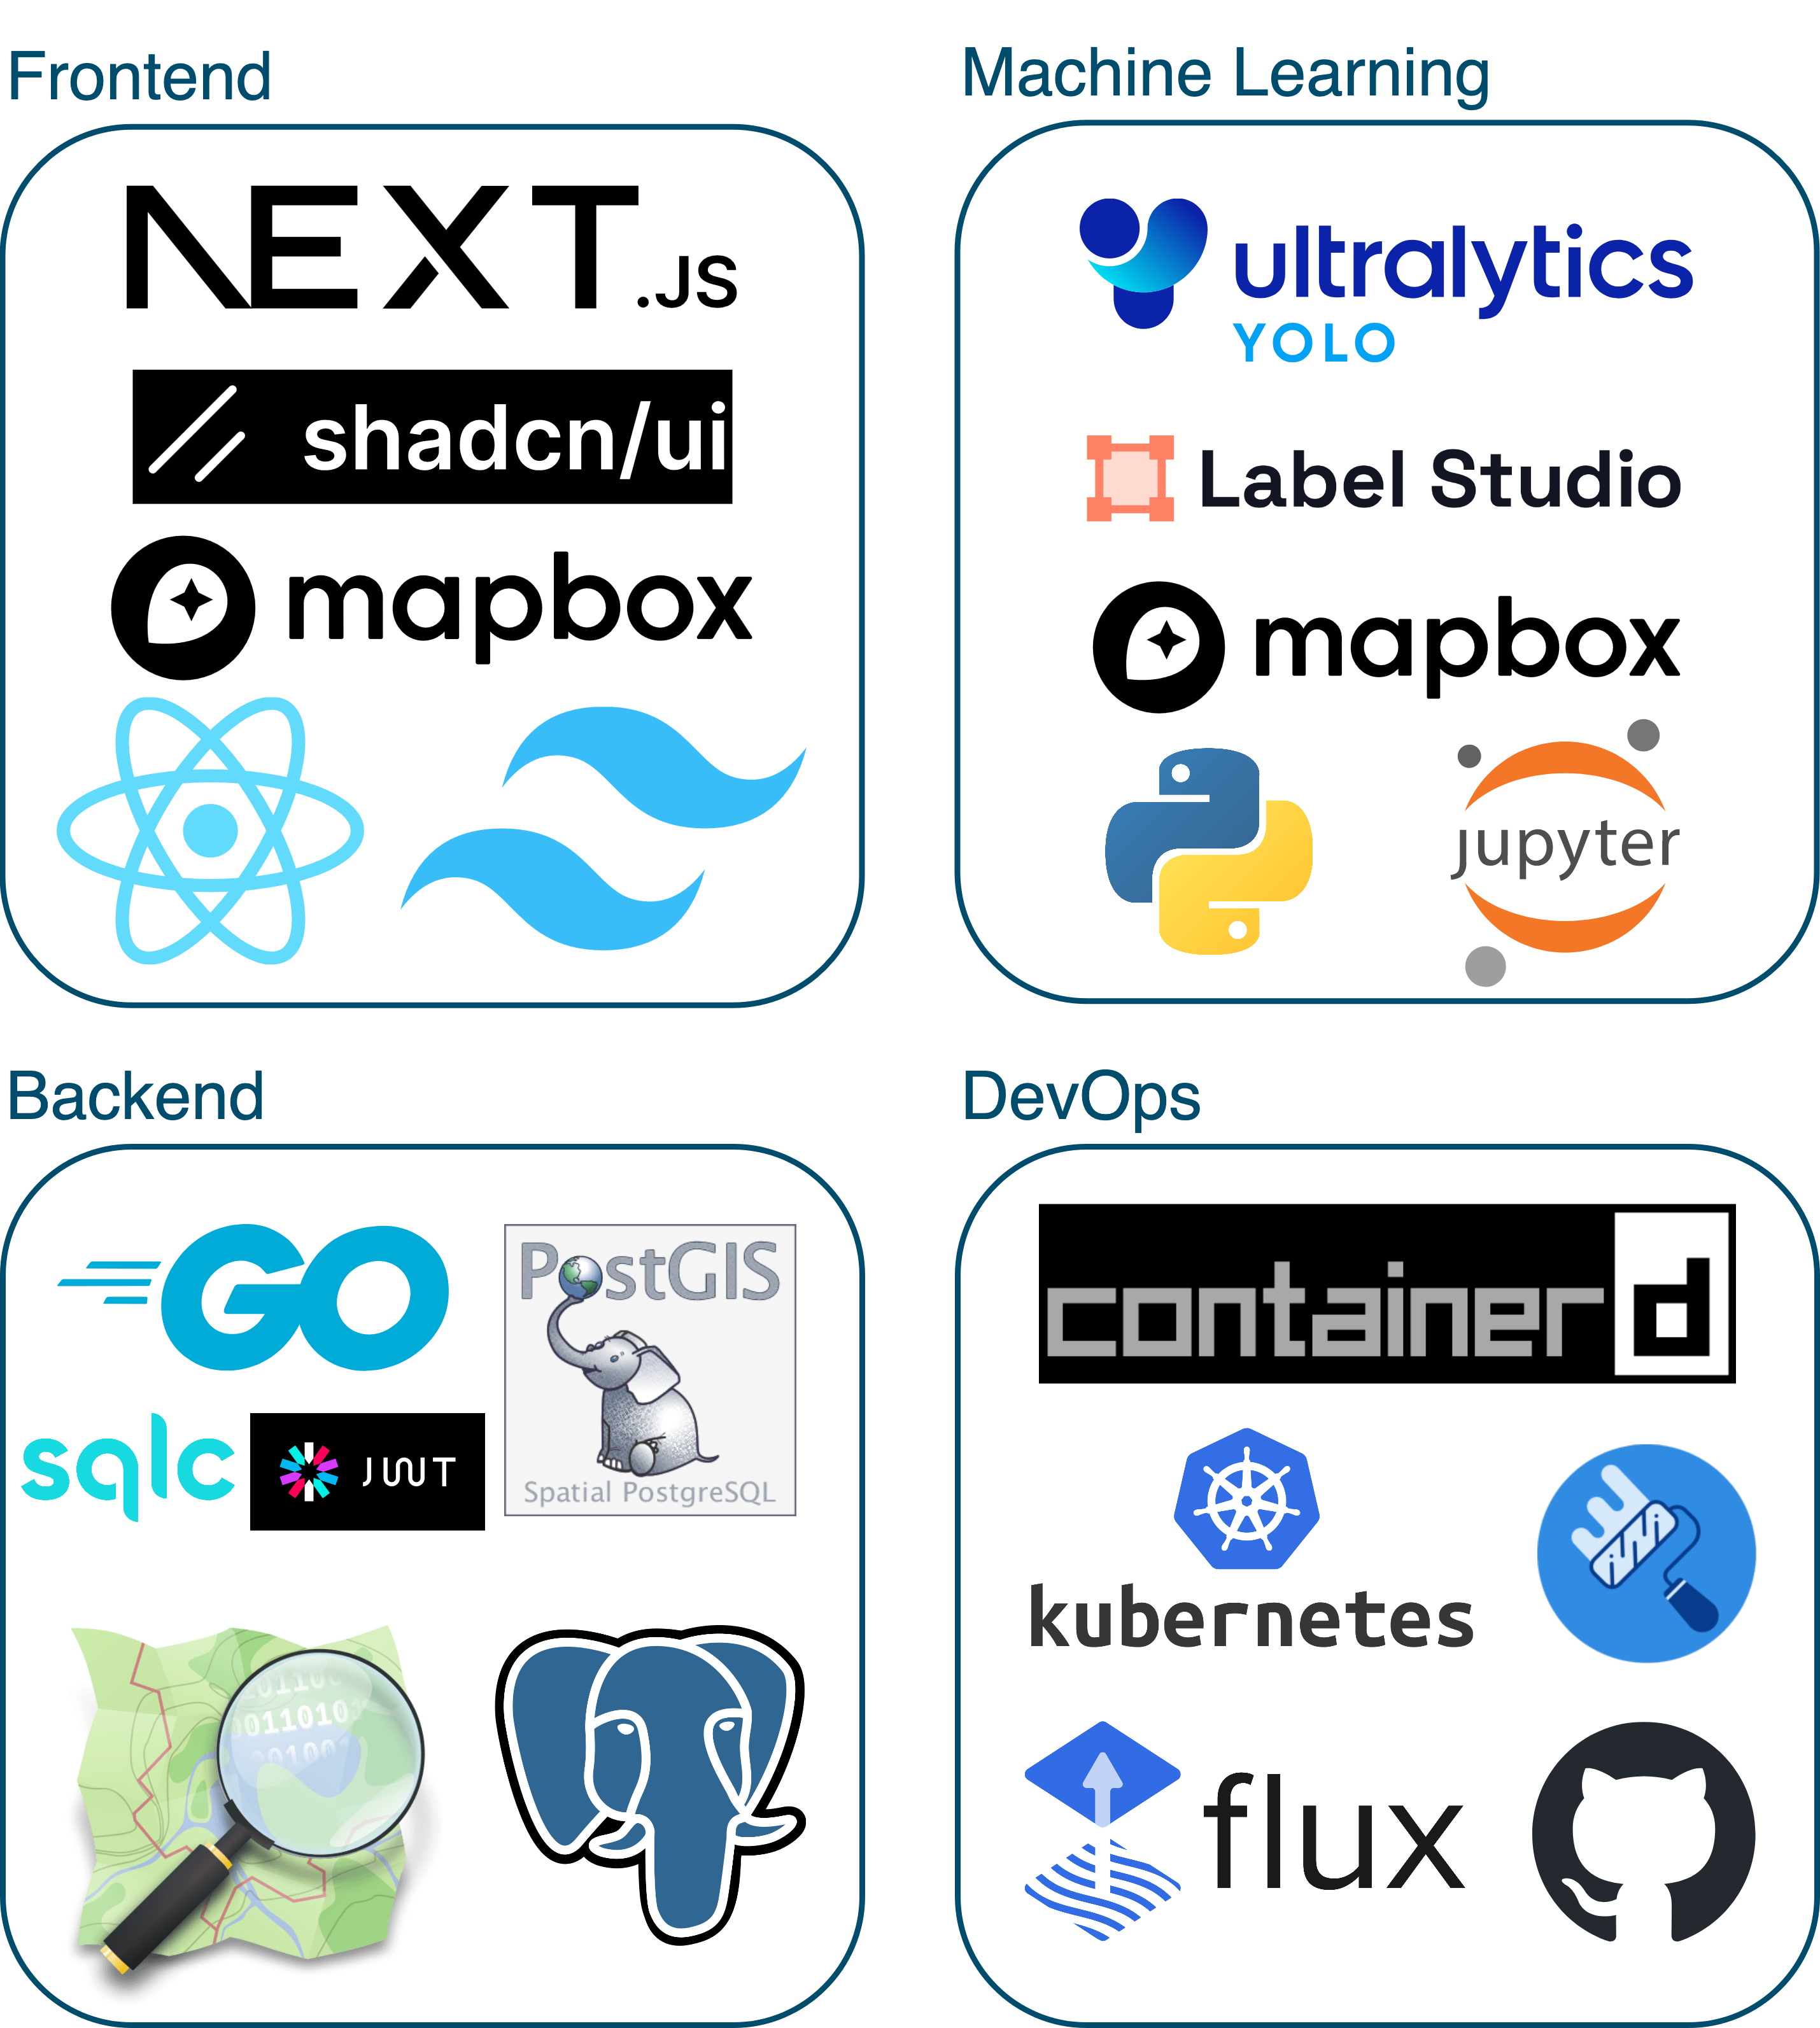
\includegraphics[width=\textwidth]{images/stack_grid.png}
    \caption{Our technology Stack}
\end{figure}

The frontend stack plays a critical role in providing a smooth and interactive user experience for the application. It is built on top of modern web technologies, each serving a unique purpose:

\begin{itemize}
    \item{} \textbf{Next.js:} This React framework offers server{-}side rendering (SSR) and static site generation (SSG), which improve performance, SEO, and user experience.
    \item{} \textbf{React:} As the foundation of the frontend, React allows for component{-}based development, making the interface scalable and easy to maintain.
    \item{} \textbf{TailwindCSS:} A utility{-}first CSS framework that simplifies styling by providing ready{-}to{-}use classes, enabling rapid UI development.
    \item{} \textbf{shadcn/ui:} A collection of reusable UI components that work seamlessly with Next.js and React, enhancing productivity and consistency across the application.
    \item{} \textbf{Mapbox:} A powerful mapping platform that enables interactive, customizable maps. It helps visualize geospatial data effectively, which is key for location{-}based services in this project.
\end{itemize}

These technologies combine to create an engaging user interface that is both functional and visually appealing, allowing users to interact with location{-}based data and services efficiently.
